\section{Introduction}\label{introduction:introduction}

In this project, we aim to explore how Cassandra, a distributed database, handles different types of client-centric consistency observed by applications. The consistency models to be tested are read-your-writes (RYW), monotonic-reads (MR), monotonic-writes (MW), and writes-follow-reads (WFR)~\cite{terry1994}. We first set up a replicated distributed database with three Docker containers forming a Cassandra cluster, then explored its consistency behaviours by tuning the read consistency level, the write consistency level~\cite{cassandra-dynamo}, and artificially injected replication latency. For each consistency model, we first derive a prediction based on the condition R + W \textgreater{} N, then construct a test in which a single client writes and reads through different coordinator nodes, and finally measure the fraction of trials that violate the guaranteed consistency.

Note that the tests are repeated under several settings, including normal, one node failure, and a network partition that blocks an individual node, to represent different levels of network availability. Our results show that delayed propagation exposed read-your-writes and monotonic-reads violations under weak consistency settings, while stronger settings prevented these observed anomalies in successful trials but reduced availability during failures and partitions. In the monotonic-writes and writes-follow-reads tests, deliberately inverted timestamps caused earlier values to prevail over later updates, even at stronger consistency levels. These findings highlight the distinct roles of replica visibility, availability, and timestamp ordering within the tested workloads, rather than establishing general consistency guarantees.

\subsection{System Configuration}\label{introduction:system-configuration}

{
\begin{table}[H]
\centering
\small
\renewcommand{\arraystretch}{1.15}
\caption{System configuration and software environment.}\label{tab:introduction-1}
\begin{tabular}{@{}
  >{\RaggedRight\arraybackslash}p{(\linewidth - 2\tabcolsep) * \real{0.2300}}
  >{\RaggedRight\arraybackslash}p{(\linewidth - 2\tabcolsep) * \real{0.7700}}@{}}
\toprule\noalign{}
\begin{minipage}[b]{\linewidth}\RaggedRight
Component
\end{minipage} & \begin{minipage}[b]{\linewidth}\RaggedRight
Configuration
\end{minipage} \\
\midrule\noalign{}
Host & Lenovo Thinkbook 16p, Linux {[}6.18.33.2-microsoft-standard-WSL2 x86\_64{]}, Docker {[}29.7.2{]}; Macbook Pro, Darwin 27.0.0 arm64, Docker {[}28.4.0{]} \\
Database & Apache Cassandra {[}4.1.12{]} \\
Client & Windows/WSL2: Python {[}3.11.16{]}, macOS: Python {[}3.12.2{]}; Cassandra-driver {[}3.30.1{]} both \\
Keyspace & consistency\_lab, replication factor=3, SimpleStrategy \\
Table & kv(key text PRIMARY KEY, value int, writer text) with read\_repair=NONE, speculative\_retry=NONE~\cite{cassandra-read-repair,cassandra-ddl} \\
Consistency Levels & ONE, QUORUM, ALL (requiring responses from 1, 2, and 3 replicas, respectively; $N=3$). \\
\bottomrule
\end{tabular}
\end{table}
}

Here, we disabled two default settings, read repair and speculative retry, because both would mask the divergence we want to observe. Read repair writes the newest value back to stale replicas as part of a read request, so a violation seen once would be repaired before we could observe it again. Speculative retry will try to contact extra replicas when one responds slowly, which the injected latency would trigger constantly, making CL=ONE behave just like a larger CL.

In particular, to make the role of each node in the cluster clear, each client session is pinned to a chosen node through a white-list mechanism~\cite{driver-policies}. This allows us to identify and keep track of the coordinator for every read/write request.

\subsection{Cluster and Network Setup}\label{introduction:cluster-and-network-setup}

The cluster consists of three containers (cass1, cass2, and cass3) on one Docker bridge network, with cass1 serving as the seed node. Each node's CQL port 9042 is published on the host as port 9042, 9043, and 9044, respectively. The nodes communicate with one another through port 7000 inside the bridge network.

We initialize the experiment with \verb|scripts/bootstrap.sh|. It starts the cluster using Docker Compose, waits for the containers to become healthy, and checks their status with \verb|nodetool|. It then runs \verb|scripts/setup_keyspace.cql| on cass1 to create the \verb|consistency_lab| keyspace and the \verb|kv| table, retrying if Cassandra is not yet ready. The script creates a Python virtual environment in \verb|.venv|, installs the packages in \verb|requirements.txt|, tests the client connections, and records the software and host information in \verb|results/environment.txt|.

After bootstrap, we use \verb|scripts/inject_latency.sh| to apply Linux \verb|tc/netem| delay to outgoing traffic destined for port 7000 on each container. The default setting is 200 ms of delay with 50 ms of jitter. This affects internode communication, including replication and internode read traffic, while leaving the client-facing CQL ports untouched. Delaying client traffic could add time between a completed write and the subsequent read, allowing more time for propagation and changing the measured violation rate.

A node failure scenario is realized by simply stopping cass3. Meanwhile, a network partition is realized by dropping traffic on port 7000 between cass3 and the other two nodes in both directions, leaving cass3 running with its client port accessible; clients can therefore access both the majority side (cass1, cass2) and the minority side (cass3).

Finally, as we aim to emulate replication delay and node partitions rather than independent machine failures, we run all three containers on a single physical host, sharing the same system clock, within Docker Desktop's Linux environment, while the client runs directly on the host operating system.

\begin{figure}[H]
\centering
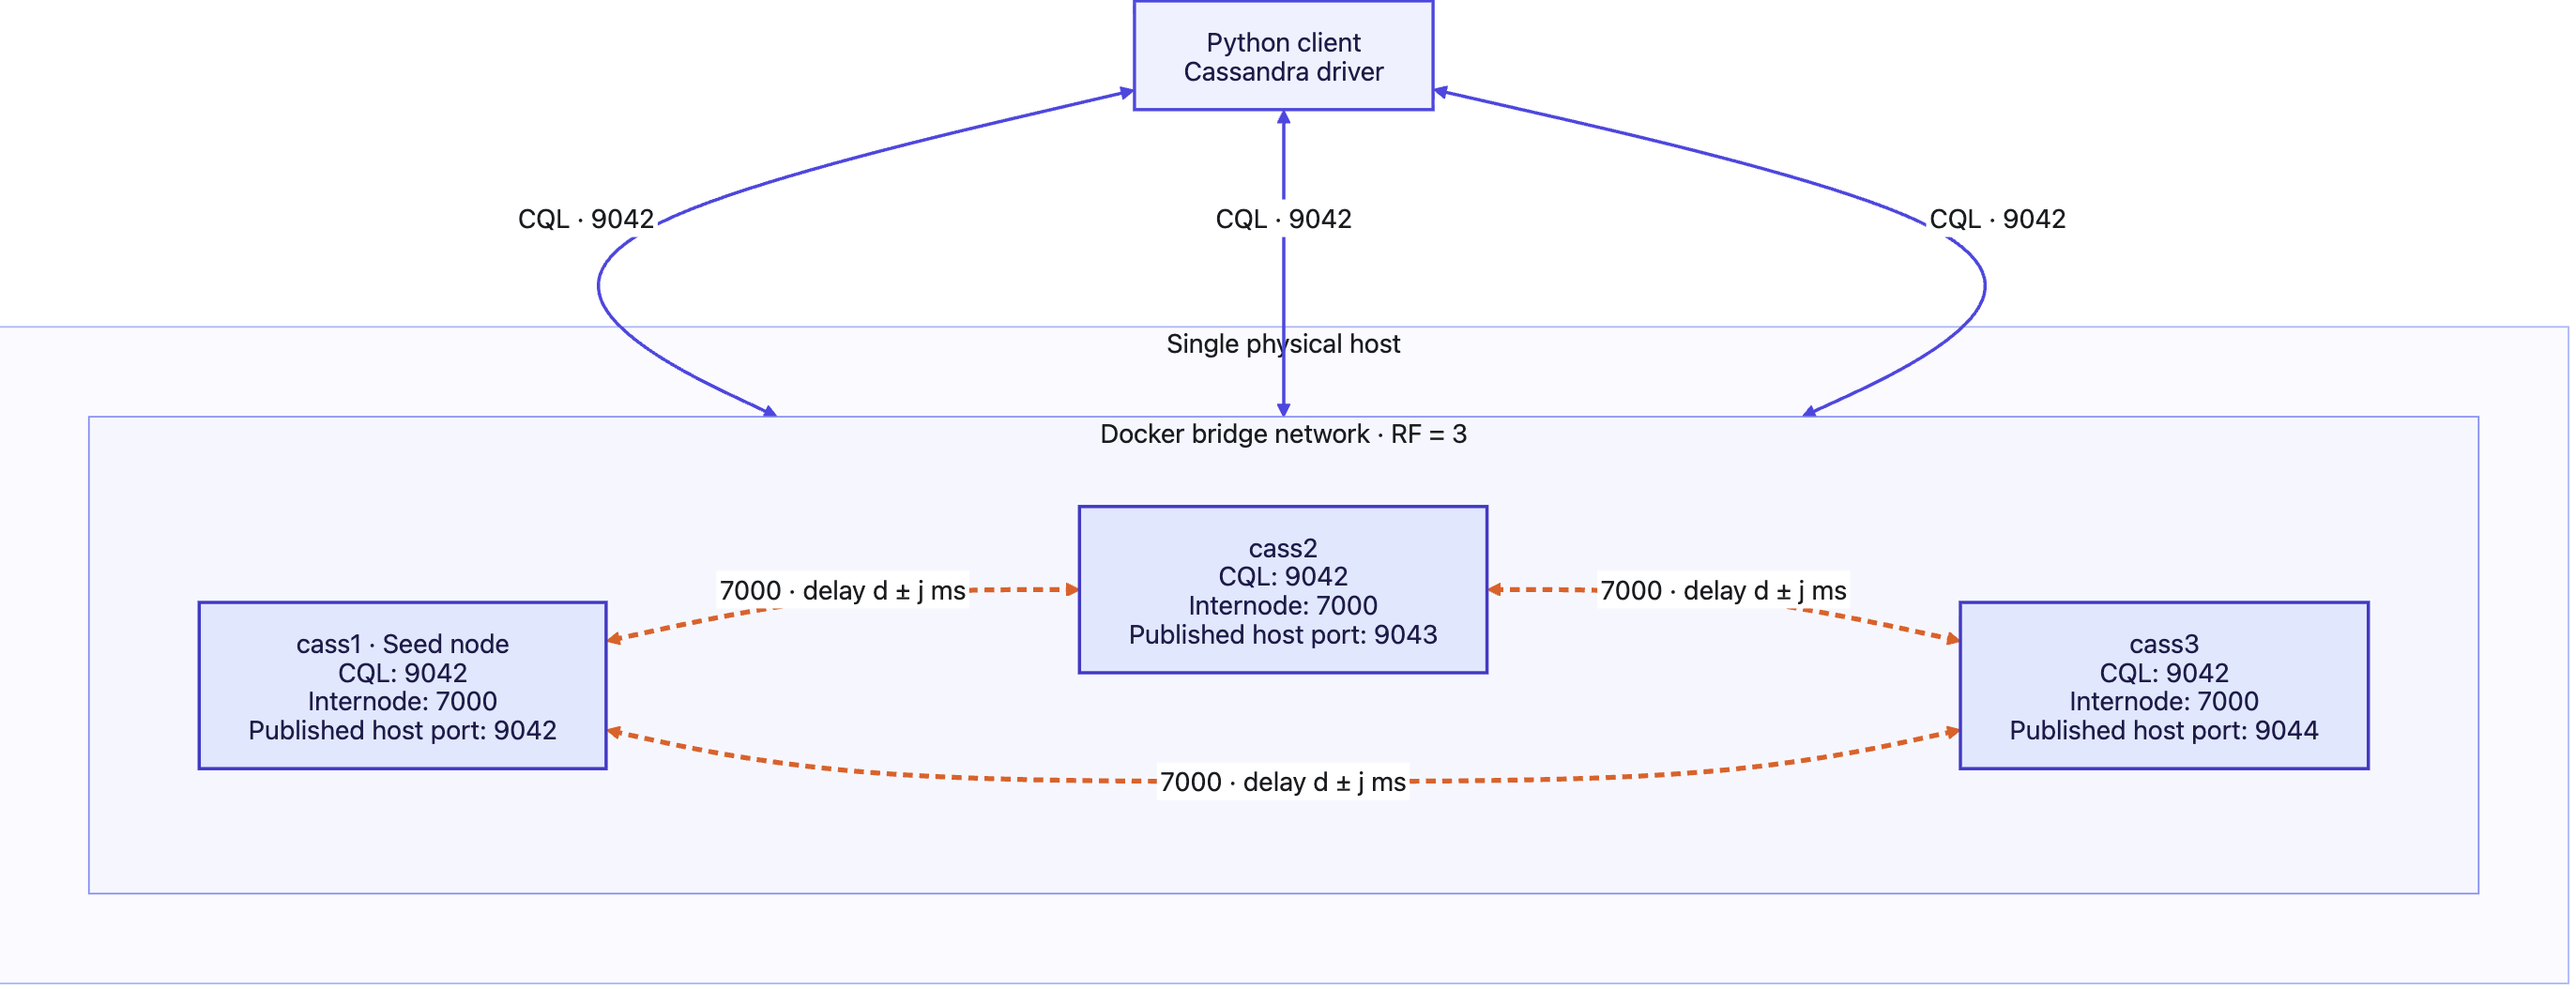
\includegraphics[width=\linewidth]{figures/architecture.png}
\caption{Three-node Cassandra cluster and communication ports.}
\label{fig:architecture}
\end{figure}

\section{Consistency Test}\label{introduction:consistency-test}
